\section{Produkt beskrivelse}
%Systemet skal kunne lagre og indlæse beskeder til og fra et eksternt socialt medie, hvilket vil spille den stor rolle i 
% Beslutninger
% Fokus på kravene, nævn dem med nummerering
% Måske som seraperat latex section
% let oprids af de etikke dilemmaer i projektet
% teknologierne
% det sociale medie som et mellemled, for at steganografere beskederne i mængden af meget andet indhold


\section{System design}
% Hvilke problemer er der ved systemet?
Ud fra kravspecifikationen bliver systemet pålagt at være sikkert, men samtidig også at køre med en fornuftig indlæsnings tid. Disse krav kan  modarbejde hinanden på flere forskellige måder, blandt andet i spørgsmålet om systemet skal køre centralt eller decentralt.

\subsection{Central eller decentral løsning}
Hvis man har spørgsmålet med optimal indlæsnings tid i mente, så vil en central løsning med en server der lagrer stien til alle beskeder i systemet. Dette gør enheder der tilgår den centrale database i stand til at forespørge og finde opslag meget hurtigt, da den har kortlagt alle relevante opslag. Dette står i modsætning til en decentral løsning, hvor brugernes enhed fungerer som mikro servere der selv skal søge efter de relevante opslag. Den søgning kræver langt flere server anmodninger decentralt, da den centrale kortlægning ikke er tilgængelig. De mange anmodninger vil resultere i længere indlæsnings tid.

\begin{figure}[H]
    \begin{subfigure}{0.5\textwidth}
        \centering
        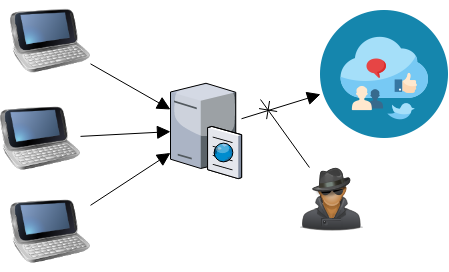
\includegraphics[width=1\linewidth, height=4cm]{Projectdoc/Assets/Illustrationer/Security_diagram_1.png} 
        \caption{Central server}
        \label{fig:central_server}
    \end{subfigure}
    \begin{subfigure}{0.5\textwidth}
        \centering
        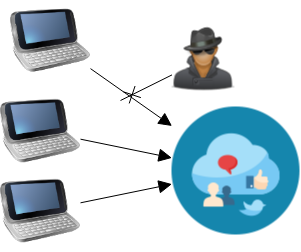
\includegraphics[width=0.7\linewidth, height=4cm]{Projectdoc/Assets/Illustrationer/Security_diagram_2.png}
        \caption{Klient-baseret system (decentral)}
        \label{fig:decentral_server}
    \end{subfigure}
    \caption{Forskellen på central og decentral server struktur}
    \label{fig:serverstruktur}
\end{figure}

En central server trods dens eventuelle positive egenskaber, udgøre dog også et potentielt sikkerhedshul, hvis denne server ikke er sikret tilstrækkeligt. Med andre ord lægger dette en systemvedligeholdelse byrde på dem der administrerer systemet. F.eks. kunne en sådan server, (Illustreret ved [Figur \ref{fig:central_server}]), lække generelle lagerede informationer, eller ligefrem blive overvåget for kommunikation, samt blive spærret som en helhed. Dette vil selvfølgelig også kunne ske for den enkelte bruger [Figur \ref{fig:decentral_server}], men disse ville i sådanne tilfælde også kun påvirke den enkelte, og ikke systemet som en helhed.
\\\\
%\textbf{Argumenterne for en delvis decentral løsning}\\
Jo mere et givet system afhænger af bestemte nodes, jo vigtigere er det at sikre disse nodes, både i forhold til DoS angreb, men også i forhold til kompromittering af bruger data. På den anden side, vil anvendelsen af servere i et centralt systemet også tillade en langt højere effektivitet. Derfor vil forskellige aspekter af kommunikationsplatformen blive videre diskuteret for at kunne finde et kompromis mellem helt centraliseret og helt decentraliseret.\\

\begin{figure}[H]
    \begin{subfigure}{0.33\textwidth}
        \centering
        \includegraphics[width=1\linewidth, height=4cm]{Struktureret_System_Udvikling/Workshop_2/Assets/} 
        \caption{Central server}
        \label{fig:central_server}
    \end{subfigure}
    \begin{subfigure}{0.33\textwidth}
        \centering
        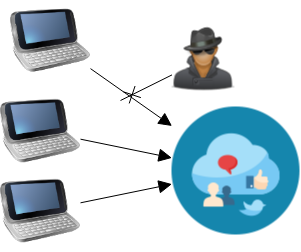
\includegraphics[width=0.7\linewidth, height=4cm]{Projectdoc/Assets/Illustrationer/Security_diagram_2.png}
        \caption{Klient-baseret system (decentral)}
        \label{fig:decentral_server}
    \end{subfigure}
    \begin{subfigure}{0.33\textwidth}
        \centering
        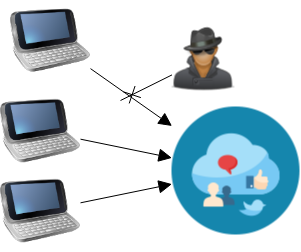
\includegraphics[width=0.7\linewidth, height=4cm]{Projectdoc/Assets/Illustrationer/Security_diagram_2.png}
        \caption{Klient-baseret system (decentral)}
        \label{fig:decentral_server}
    \end{subfigure}
    \caption{Forskellen på central og decentral server struktur}
    \label{fig:serverstruktur}
\end{figure}

For at kunne opretholde en mængde af bots, her forstået som anonyme brugere på sociale medier genereret af systemet, der har til opgave at sikrer anonymitet for brugeren på kommunikationsplatformen, associeret med en potentielt mistænkelig opførelse, vil det være nødvendigt at kunne tilføje nye bots til netværket løbende, samt opdatere status af nuværende bots, da det kunne formodes at ejerne af det relevante sociale medie ikke ønsker systematisk genereret anonyme brugere. Én mulig måde at holde styr på disse informationer kunne være at holde en database opdateret med information om de enkelte bots på de sociale medier, omhandlende om de stadigvæk er aktive, eller om de er blevet banlyst af det sociale medie, f.eks. for ikke at være en "normal" bruger. Hvis en given bot så blev lukket ned, ville den opdaterede database, gøre enhver bruger i stand til blot at vælge en anden bot. Denne løsning tilfører dog et element, en database, som vil være et kritisk led i, at tilbyde yderligere anonymitet til brugeren. Hvis denne database så ikke er tilgængelig, ville denne funktionalitet være hindret, i det at bots vil kunne blive taget ned i mellemtiden, uden at brugeren vil vide det, før brugeren får en fejlmeddelelse. Endnu værre kunne kompromitteringen af denne database gøre det muligt for uvedkommende at læse beskederne sent igennem systemet. Dette vil især være væsentligt hvis der er anvendt kryptering som ekstra sikkerhed på beskederne. Disse krypteringsnøgler vil så skulle gemmes et sted hvor alle de egentlige bruger kan få fat i dem. Derfor vil sikringen af sådan en database være vigtig. Såfremt denne database kun kontaktes for at få listen opdateret, vil trafikken imellem den og klienterne dog være begrænset. Man kunne også forestille sig en ekstra database, som kun vil blive kontaktet hvis den primære er inaktiv, og at denne database kender til andre databaser, der er backups af den primære. Denne opbygning vil gøre det meget svært at lukke systemet i længere tid. På den anden side vil dette opsætning også kræve mere hardware og mere vedligehold i form af synkronisering og opdatering osv. Dermed vil en opsætning af en sådan backup koste systemadministratoren mere og vil derfor kræve en vurdering af, om det er investeringen værd.\\
En måde at undgå dette databaseproblem, er at lade hver klient have en lokal liste over aktive bots. Denne liste vil så med jævne intervaller blive opdateret igennem klient opdateringer. Med denne fremgang er det tænkeligt, at systemet vil kræve mange opdateringer, eller at der ofte vil være et antal utilgængelige bots på listen.
\\\\
%\textbf{Argumenterne for en central løsning}\\
Som førnævnt vil et centraliseret system betyde at hele systemet vil hvile på en node, hvilket vil betyde at en angriber blot skal tage et led ud for at kollapse hele systemet. En måde hvorpå man kunne sikre systemet under en central server, er ved at lagre krypteringsnøgler på serveren, der skal hentes for at kunne læse en besked. Denne centrale server bliver det eneste led som en ondsindet angriber skal lægge ned, for at gøre hele platformen ubrugelig. Dette vil faktisk sikre brugerne, såfremt angriberen ikke kompromitterer krypteringsnøglerne. Brugernes beskeder vil være ulæselig for en angriber uden de krypteringsnøgler. Dette kan sammenlignes med en indbygget selvdestruktion af systemet.\\
Et centraliseret system vil altid kunne opdateres løbene, i modsætning til den decentraliseret løsning hvor brugerne enten er fastlåst med software der potentielt er defekt eller skal hentes på ny. Løbene opdateringer til systemet er essentielt når det sociale netværks bot konti der benyttes, ikke fungerer som tiltænkt. Dette kan ske på mange forskellige måder: Blandt andet kan de enkelte bots blive taget ned for mistanke for falsk bruger eller netværket kunne ændre sin struktur fra en ene dag til den anden. Muligheden for løbene opdatering er også essentiel ved en mulig skalering af systemet, blandt andet når systemets netværk af bots ikke kan betjene en voksene brugerbase eller når denne brugerbase ændret behov der kræver at det fundamentale system gennemgår strukturel redesign.
\\\\
\textbf{Samlet konklusion}\\
Selvom en komplet decentraliseret løsning lyder godt på papiret, så vil det udløse så mange fundamentale problemer at systemet vil være bøvlet og potentielt ubrugeligt. Da systemet afhænger så kraftigt på en trejdeparts service, så vil små ændringer så som:
\begin{itemize}
    \item[-] Systemets bot netværk kan blive delvist eller helt lukket ned. Dette kan ske af mange forskellige grunde blandt andet ved brud på det sociale medies ToS (Terms of Service) eller ved en eventuel afsløring af hele systemet / projektet. 
    \item[-] Tredjeparten kan ændre deres API struktur på sådan vis at det fundamentale system ikke længere fungerer som tiltænkt.
    \item[-] At danne et ekstra lag af sikkerhed, ved anvendelse af krypteringsnøgler, vil være meget nemmere med en central løsning.[-] 
    \item[-] Den decentrale løsning vil ikke kunne lukke alle brugernes tilgang på sammetid, da der ikke er nogen central database.
    \item[-] Det vil kræve løbende opdatering af klienterne, at holde listen af aktive bots fuldt funktionel.
\end{itemize}

% En samling af decentral og central løsninger

% delkonkusion Central eller decentral
% teknisk svær opgave

\subsection{Sammenkobling af beskederne}

- Hvordan kan vi skulle sammenkædnings nødvendig data i metadata?

\\\\
\textbf{Privat beskeder}\\

%- Hvordan kan man sikre en fornuftig køre tid? (Undg̊a 10000 undersøgelser for at finde  ́en kommentar)
%- Formindsk chancen for mistænkelig data trafik. B̊ade i server requests og det visuelt uploaded
%— Load tid

% - Med kun bots
% -- Request mængde
% -- API afhængighed

% - Bruger login
% -- Bruger sikkerhed

% - Samlet løsning med måde bot og bruger

\subsection{Opsummering af alle overvejelserne}
% Her beskrives det komplette system
% På numre ind i figuren, og måske den skulle opdateres til at ligne mere den på tavlen!
\begin{figure}[H]
    \centering
    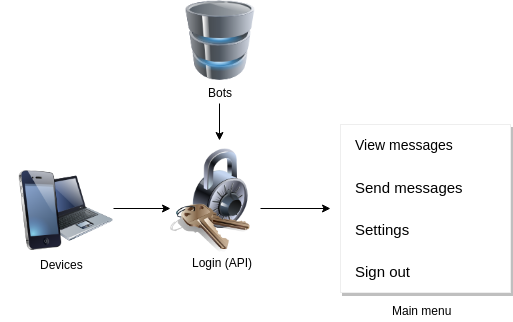
\includegraphics[width=0.70\linewidth]{Projectdoc/Assets/Illustrationer/simple-system.png}
    \caption{System}
    \label{fig:sysdiagram}
\end{figure}

Systemet beskrevet ved [Figur \ref{fig:sysdiagram}] er baseret på en brugers aktive handlinger, og kan derved styres fra et centralt sted. Her tales om enten brugerens egen enhed, eller en central server, der ikke fortager andre handlinger end at responderer klart på en brugers kommandoer.

I systemets handlings diagram ovenfor [Figur \ref{fig:sysdiagram}] ses produktets overordnede handlingsflow. Diagrammet er ikke en endelig eller færdig udarbejdelse, men skabt til at give et letforståeligt overblik over systemets indhold, nødvendige resurse behov, samt mulige anvendte teknologier. Ud fra diagrammets flow, med start fra den sorte cirkel i toppen, kan der som et eksempel ses, at systemet anses for at skulle have tilgang til en Database, indeholdende mulige Bot associeringer til en brugeres login, eller en tilgang til det anvendte sociale medies API for samme.\\
I dette eksempel er f.eks. ikke videre beskrevet hvordan, eller om systemet overhovedet skal, håndtere denne databases placering eller tilgang, efter en eventuel spærring fra tredjeparter, der f.eks. kunne anse systemet for at understøtte maliciøse aktiviteter.\\
Efter denne login aktivitet ses hovedmenuen, hvorfra brugerne kan vælge at f.eks. tilgå systemets indstillinger, danne en ny besked, eller hente tidligere beskeder og tråde. Denne lægger også op til et andet dilemma omhandlende hvordan systemet, uden at skabe en større række af mistænkelige forespørgsler, skal kunne genkende, hente, og sammekæde flere beskeder på op til flere mulige brugere kontoer, hvilket efter simple normale requests vil kræve op til måske flere hundrede transmissioner per request.\\
Senere i dette afsnit vil disse føromtalte dilemmaer såvel som, teorier og tanker blandt andre blive videre redegjort for, med henblik på at skabe et endeligt oplæg til en række tekniske læsningsforslag.

%\subsection{Teori}
%Dette afsnit vil redegøre for de grundlæggende teorier og begreber bag systemets komponenter. Afsnittet vil lægge op til en række tekniske løsningsforslag, som kræver den viden beskrevet i dette afsnit.

\subsubsection{API, REST og Socket kommunikation}
De fleste tjenester opsat i dag, foruden deres givende handlinger, tilbyder også mulighed for at et program automatisk kan foretage interaktion, altså uden et menneskes handlinger. En sådanne maskin interaktion siges, at anvende et API (\underline{A}pplication \underline{P}rogramming \underline{I}nterface) til at standardisere dets forventede inputs og udputs. 
API står i modsætning til UI (\underline{U}ser \underline{I}nterface), hvor et menneske interagerer med en tjeneste, og beskriver hvordan, samt hvad der skal til, for at foretage bestemte handlinger, så som f.eks. efter denne rapports idé, at uploade et billede til en given tjeneste. En API er derfor generelt nødvendig for at kunne opsætte en troværdig interaktion mellem tredje parts tjenester, og den oprindelige udbyder. \cite{WhatIsAPI}

"API" er i dag en alment kendt metode betegnelse, og findes derfor i et utal at forskellige versioner, typer og udgivere. F.eks. er nogle af de mest kendte Googles eget API "Google-API", eller det mere standardiserede web API "REST" (\underline{RE}presentational \underline{S}tate \underline{T}ransfer), begge ikke kun anvendt i lukkede systemer, men også generelt alment på nettet. \cite{codecademy_REST}

En API protokol beskriver kun hvordan en given data forventes formateret, og ikke hvordan en data skal leveres, derfor anvender mange tjenester også en eller anden form for Socket kommunikation til at forventningsafstemme, og sikre en data leverance. Bagsiden ved opsætning af en Socket forbindelse er dog at disse også kræver opsætning af en listener, en server applikation, der aktivt står og lytter efter en klient, som ønsker at oprette en kommunikation på en given port, dette vil sige at den oprindelige tjeneste, efter opsætningen af et socket, nu har et åbent interface, og derved også en øget sikkerheds risiko. Efter opsætningen er listenerens opgave at sørge for hurtigst muligt, at sikre en åben forbindelse på en anden port, mellem denne server og klient ved en oprettet forbindelse, da porten for listeneren igen skal være fri til den næste klient. \cite{WhatIsSocket} Selv om man ikke direkte kan undgå brugen af Socket kommunikation, ved en server til klient kommunikation, og derved generelt må acceptere denne øgede sikkerheds risiko, forefindes der dog stadig flere måder at opnå samme resultat, også uden direkte opsætning af selve socket forbindelsen, så som foreksempel HTTP-REST, Active-MQ eller Rabbit-MQ. \cite{SocketAlternatives}

\subsubsection{Metadata}
\label{Metadata}
På projektets sikrede kommunikationsplatform vil det være nødvendigt at kunne finde sammenhængende beskeder og denne sammenkædning vil ikke kunne foregå på åbenlys vis på et socialt medie. I stedet kunne én mulighed være, at gemme sammenhængen i noget tilsyneladende uskyldig metadata, men som er genereret ud fra en prædefineret algoritme. Dette vil give den sikrede kommunikationsplatform noget specifikt at søge efter, uden at det vil være et let læseligt flag. Men hvad er metadata?\\\\
Metadata kan grundlæggende defineres som data om data. Dermed kan det anvendes i mange sammenhænge. Et eksempel kunne være et billede. Dataen i et billede er i simpleste forstand lysintensiteter, i sort/hvid billeder, eller farver. Men udover denne data kunne man også gemme ting som dato, klokkeslet, GPS koordinater, navnet på ophavsmanden osv. Alt dette er eksempler på metadata som ikke påvirker indholdet, men som gør indholdet mere brugbart i mange forskellige sammenhænge. For eksempel vil vedhæftede søgeord gøre et billede galleri meget mere effektivt i at præsentere det ønskede materiale. Metadata kan både genereres automatisk af hardware/software systemer, men en bruger kunne også tilføre metadata manuelt.\\ Dette er især sandt på sociale medier hvor der kan findes en stor mængde af generelle søgeord. Netop det faktum at sociale medier tillader de enkelte brugere at skabe en varierende mængde af metadata for et hvert billede, sandsynliggør at systemet vil være i stand til at generere disse søgeord med en prædefineret algorimte for hver tråd på forummet. Dette vil så gøre det muligt at søge efter nye opslag på enhver forumstråd.



\subsection{System design proces / diskussion}
% Top:
%Beskrivelse af vores tilgang til dette afsnit, med de overordnet spørgsmål og flere løsningsforslag
% Hvilke problemer er der ved systemet?

\subsubsection{Sammenkædning af beskeder}

\textbf{Forslag 1: Lagring af den hemmelige besked på brugerens profil}
\begin{figure}[H]
    \centering
    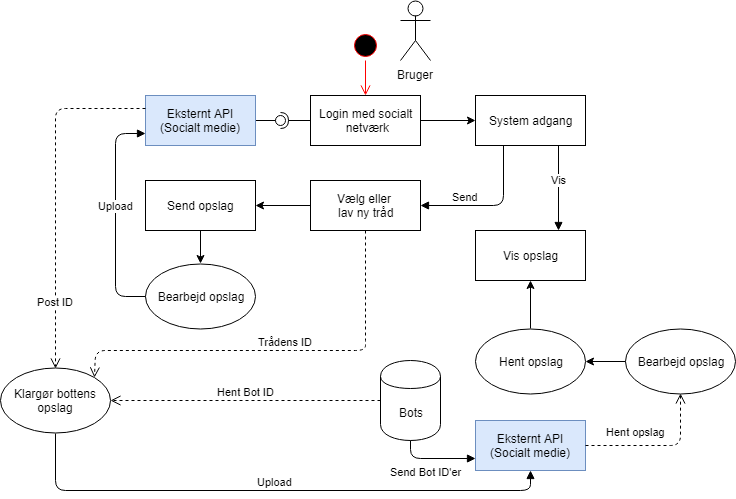
\includegraphics[width=0.8\linewidth]{Projectdoc/Assets/Illustrationer/userbased-system.png}
    \caption{UML diagram over et brugerkonto baseret kommunikations system}
    \label{fig:userbased}
\end{figure}

Brugerne logger ind på platformen [Figur \ref{fig:userbased}] ved hjælp af deres egne kontooplysninger til et given socialt medie. Platformen har nu mulighed for at sende den hemmelige besked direkte til brugerens egen konto. Platformen lægger automatisk den hemmelige besked ind i den pågældende bruger's opslag, og returnere samtidigt opslagets unikke ID tilbage. Dette ID bliver sammen med et unikt tråd ID lageret på en bot. Tråd ID bliver enten generet på stedet, hvis der oprettes en helt ny tråd, eller så bliver et tråd ID nedarvet fra et tidligere ID. Botten har også en konto på det givne sociale medie, kontrolleret af platformen selv. 

Når brugerne af platformen ønsker at få alle opslag vist, så henter systemet alle bots oplag i den rækkefølge som opslagene er tilsendt til botten. Botten har, som før nævnt, gemt data i disse opslag som: tråd struktur og adressen (PostID'et) på beskeden. Det ekstraheret postID kan nu spores tilbage til den bruger der ejer den hemmelige besked.
\\\\
\textit{Fordele:}
\begin{itemize}
    \item[+] \textbf{Brugerkonti som proxy} \hfill \\ 
    Hvis en bot bliver undersøgt vil beskederne ikke umiddelbart kunne blive aflæst. Samtidig vil det også være muligt for en bruger at genskabe deres opslag ved en eventuel nedlukning af en bot.
    \item[+] \textbf{Sammenkædning af posts af samme forfatter} \hfill \\ 
    Med et system som dette hvor opslag hentes fra brugerne selv, kan man samtidig hente og hashe brugerens ID, sådan måde at det ikke kan linkes tilbage til brugeren sig, men indikere at den samme bruger står bag flere opslag.
\end{itemize}
\\
\textit{Ulemper:}
\begin{itemize}
    \item[-] \textbf{Skjul af metadata} \hfill \\
    Denne løsning kræver at en rækker ID'er bliver skjult i metadata på sådan vis at det er genkendeligt for systemet, men ikke mennesker. Et problem der på nuværrende tidspunkt ikke har en løsning.
    \item[-] \textbf{Dobbelt forspørgelse} \hfill \\
    Systemet skal foruden kontakte systems egne bot konti også kontakt den enkelte bruger der opbevare et opslag.
    \item[-] \textbf{Begrænset kontrol over opslag} \hfill \\ 
    Brugeren kan slette deres opslag udenom systemet, og ødelægge trådes struktur.
\end{itemize}

%\textbf{Doubly linked list (Algoritme)}

% - Central server / server cache (Sikkerheds brist)

\subsubsection{Næste emner}
\\
- Hvordan kan man sikre en fornuftig køre tid? (Undgå 10000 undersøgelser for at finde én kommentar)\\
- Formindsk chancen for mistænkelig data trafik. Både i server requests og det visuelt uploaded\\
--- Load tid
\\
- API udbyderen som brist i systemet?\\

--- TOS problemer\\
--- Lukning af bots og dermed samtaler\\
--- Sikring ved lukning
\\
- Hvordan skal forum strukturen være ? (Design)
\\
- Hvordan kan vi skulle sammenkædnings nødvendig data i metadata?
\\
- Delkonklusion, samt endelige valg af løsning

% ==================================
% Ekstra kommentarer
% ==================================

% Foruden selve strukturen: Er der også problemer med fetching af sammenhæng?
% Kan der være et kulturelt problem i steganografi på et socialt medie?

% Så længe den primære anvendelse af systemet foregår igennem en hjemmeside, vil denne server kunne sidde med denne bot liste selv. Dette gør dog blot denne server endnu mere kritisk.

% Denne liste kunne også findes på en database som udelukkende har denne liste af bots. Dette vil minimere trafikken til databasen, hvilket vil mindske dens synlighed.

% Ingen interconnectivity mellem devices, men skal facilitere data udveksling.... How the f-ing hell?

% Dynamic updating / Databaser

%Et nyt problem når spørgsmålet om login håndtering bliver rejst, og om hvorvidt forbindelsen med det sociale medie skal foregå ved hjælp af systemgeneret konti eller brugerens egen konto.

% På en central server er der også mulighed for at forebygge tung belastning og f.eks. indlæse, samt gemme (som en slags cache), alle beskeder for en specifik tråd, inden brugeren faktisk beder om dens indhold. Derved kan man benytte serverens hviletilstand til aktivt at forebygge aktiviteter, og derved mindske fremtidige belastnings problemer.

%Grundet disse negative effekter for en central server, der generelt berører brugerens sikkerhed, vil den mest optimale løsning for projektets sikre kommunikation være, at anvende brugernes enkelte enheder til system håndtering. Dette vil dog ikke i sig selv kunne tages til konklusion, da et system baseret alene på enkelte enheder egen håndteringer, vil kunne danne en større kompromitterings fare. Denne fare vil kunne opstå ved anvendelse af lokal cache for data hentning, da denne information vil kunne findes på flere nodes, dog uden denne cache vil de enkelte enheder skulle foretage mange heavy loads forespørgsler. Disse forespørgsler vil ikke bare danne større spekulation hos netværksmonitorering, og derved en større sandsynlighed for terminering, men også danne et meget stort dataforbrug hos enddevices, samt en lang indlæsnings tid, der kan fremprovokere brugerfejl.